\documentclass{article}
\usepackage{graphicx} 
\usepackage{float}
\usepackage{booktabs}
\usepackage{array}
\usepackage{arydshln}
\usepackage{siunitx}
\usepackage{hyperref}
\usepackage{cancel}
\usepackage{changepage}
\usepackage{placeins}
\usepackage{enumitem}


\usepackage{tabularx}
\usepackage{amsmath, amssymb, amscd, MnSymbol, mathrsfs}
\usepackage{cellspace}
\usepackage{tikz}
\usetikzlibrary{calc, patterns, angles, quotes, decorations.markings, decorations.pathmorphing, hobby}

\usepackage{chemfig}
\usepackage{caption}
\usepackage{tcolorbox}
\usepackage{bm}
\usepackage{pdfpages}
\usepackage{empheq}
\usepackage{pgfplots}
\pgfplotsset{compat=1.18}
\usepackage[oldvoltagedirection]{circuitikz}
\usepackage{microtype}
\usepackage{tikz-3dplot}
\usepackage{bibref}
\usepackage{textcomp}
% Custom commands
\newcommand{\vect}[1]{\boldsymbol{\mathbf{#1}}}
\newcolumntype{C}{>{\centering\arraybackslash}X}
\newcolumntype{M}[1]{>{\centering\arraybackslash}m{#1}}

\usetikzlibrary{external}
\tikzexternalize[prefix=figures/]


\usepackage[margin=1in, left=0.8in, right=0.8in, includeheadfoot]{geometry}
\usepackage{fancyhdr}
\usepackage{graphicx}
\usepackage{tabularray}

\pagestyle{fancy}
\fancyhf{}


\renewcommand{\headrulewidth}{0.4pt}
\renewcommand{\footrulewidth}{0.4pt}

\fancyhead[L]{
\includegraphics[height=1.2cm]{images/Kingston_University_London_logo_200-tablet.png}}
\fancyhead[R]{EG4019 - ME - Engineering Mechanics and Materials}
\fancyfoot[C]{Department of Mechanical Engineering}
\fancyfoot[R]{\thepage}

\geometry{top=0.5in,bottom=0.7in}
\usepackage{scalerel}

\setlength{\headheight}{30pt}
\setlength{\footskip}{20pt}


\usepackage[export]{adjustbox}
\usepackage{tocloft}
\renewcommand{\cfttoctitlefont}{}
\renewcommand{\contentsname}{}
\renewcommand{\cftsecleader}{\cftdotfill{\cftdotsep}}

\setlength{\cftbeforesecskip}{0.5em}


\usepackage{xurl}

\renewcommand{\theequation}{\text{Eq.}~\arabic{equation}}
%Refer to the equation as \eqref{equation}.

\begin{document}
        

    \vspace*{\fill}
    \begin{center}
        \textbf{\Huge Laboratory Report}\\[10pt]
        \LARGE \textbf{Tensile Test}
    \end{center}
    \vspace*{\fill}

    \Large    
    \begin{tabular}{@{}l l l@{}}
        \textbf{Submitted by:} & Sakariye Abiikar (Group Leader) & K2371673 \\
        & Sandeep Singh & K2314795 \\
        & Aland Floyd Noronha & K2423819 \\
        & Alan Roy & K2314478 \\
        & Judas Surname & K5671234 \\
    \end{tabular}
    
    \vspace*{\fill}
    
    \begin{tabular}{@{}l l@{}}
        \textbf{Key Dates:} & Date of practical: \\
        & Deadline: 17/12/2024 \\
        & Date of submission: \\
    \end{tabular}
    \vspace*{\fill}
    
    \large
    \newpage\noindent\vspace{2em}
    \begin{center}
        \LARGE \textbf{Contribution Table}\\[3em]
    \end{center}
    

    
    \begin{tblr}{
            colspec={Q[4cm]Q[4cm]Q[4cm]Q[3cm]},
            hlines,vlines,
            cells={valign=m,halign=c},
            rows={ht=4\baselineskip},
            row{1}={ht=1.5\baselineskip,font=\bfseries},
        }
        Student & Course & Contribution & Picture \\ 
        Sakariye Abiikar & Mechanical Engineering & Results, Theory, Recommendations & 
\includegraphics[width=2cm,valign=c]{images/profile.jpg} \\ 
        Andrew Surname & Aviation & Introduction & 
\includegraphics[width=2cm,valign=c]{images/profile.jpg} \\ 
        Lucas Surname & Astro & Results & 
\includegraphics[width=2cm,valign=c]{images/profile.jpg} \\ 
        James Surname & Mechanical Engineering & Discussion, References & 
\includegraphics[width=2cm,valign=c]{images/profile.jpg} \\ 
        Judas Surname & Civil Engineering & No Contribution & 
\includegraphics[width=2cm,valign=c]{images/profile.jpg} \\ 
    \end{tblr}
    
    \normalsize
    \newpage\noindent\vspace{1em}
    \begin{center}
        \LARGE \textbf{Table of Contents}\\[1.5em]
    \end{center}
    \tableofcontents
    \thispagestyle{fancy}


    \newpage\vspace*{-20pt}\large

    \section{Abstract}
    \vspace*{1em}
    This study investigated the effects of two thermal treatments on the mechanical properties of HE30/BS1476 aluminium alloy, initially characterized by a hardness of 120 HV5, an elastic modulus of 6 GPa, and an ultimate tensile strength of 500 MPa. The alloy underwent two heat treatments: first, heating for 90 minutes at 520\textdegree C, followed by an additional 40 minutes at 184\textdegree C in open air. Three distinct alloy variations were produced as a result of these treatments. The aim of the research was to quantify changes in hardness, modulus of elasticity, yield strength, ultimate tensile strength (UTS), and percentage elongation. Hardness was measured using a Zwick Roell ZHU hardness testing machine with a 5 kg load (HV5) (See Appendix A), and properties such as stress and strain were derived from data obtained using a Zwick Roell 2050 tensile testing machine.\\[1em]
    \textcolor{red}{Needs small info on results and reflection/conclusion (to be added at a later date)}
   
    
    \newpage\vspace*{-20pt}
    \section{Introduction}

        In engineering, the selection and optimization of materials directly impact the performance of a design application, especially in aerospace, automotive, and construction industries. \\[8pt]
        \noindent
        Aluminum alloys have a good strength-to-weight ratio and corrosion resistance; therefore, they are very important in such sectors, though mostly in applications requiring specific mechanical improvements through controlled processes. \\[8pt]
        \noindent
        Research by metallurgists such as Sorby and Sauveur demonstrated that \textbf{heat treatment} significantly improves the properties of alloys. These thermal treatments alter the alloy's microstructure, leading to enhanced hardness, elasticity, and tensile strength. Different types of heat treatments, such as solution heat treatment and quenching, are tailored to achieve specific mechanical properties depending on the alloy’s application.\\[8pt]
        \noindent
        The \textbf{aging process} is a critical aspect of heat treatment, fundamental to precipitation hardening, as highlighted by metallurgists like William Hume-Rothery. It enhances the material's properties by promoting the formation of fine precipitates, which obstruct dislocation movement, thereby increasing the alloy's strength and hardness. Aging is carefully controlled in terms of temperature and time to optimize the distribution of these precipitates, ultimately maximizing the alloy’s performance.\\[8pt]
        \noindent
        For example, one study applying these strategies involved a solution heat treatment of Al6082 alloy for 8 hours, resulting in an increase in hardness from 65 BHN to 102 BHN (See Appendix B). Additionally, its tensile strength rose from 154 MPa to 280 MPa after 6 hours of ageing at 205\textdegree C and 495\textdegree C (Singh, R., Singh, P., \& Das, 2023).\\[8pt]
        \noindent
        These microstructural enhancements allow aluminum alloys such as HE30 to be used in very demanding applications in the aerospace and automotive industries.\\[8pt]
        \noindent
        This research work investigates the response of HE30 aluminum alloy to thermal treatments by quantifying the changes in mechanical properties and in turn contributing to the optimization of materials for critical applications where performance under stress is essential. 
    
            
    \newpage\vspace*{-20pt}
\section{Method and Experimental Procedures}
The alloy samples used in this study underwent pre-treatment at an external facility, where heat treatment processes were conducted. While a brief overview of sample preparation is provided for context, detailed descriptions of the heat treatment processes are omitted, as they fall beyond the scope of this study. This section focuses exclusively on the \textbf{material testing} conducted in our laboratory.\\[8pt]
This approach ensures a focused and precise account of the laboratory work that we did, avoiding unnecessary assumptions or extrapolations.
\subsection{Method}
This laboratory research primarily focused on the evaluation of the mechanical properties of our alloy samples, specifically key metrics such as yield strength, ultimate tensile strength (UTS), modulus of elasticity, hardness, and percentage elongation. These properties are essential for understanding the material's behavior under stress and are typically used to assess the material’s suitability for different engineering applications.\\[8pt]
The methodology applied in this research was designed around an \textbf{integrated testing strategy}—an approach that aims to maximize the amount of data obtained from each step while ensuring the highest level of accuracy and efficiency. This is often referred to as \textbf{data-driven experimentation} or \textbf{multivariate analysis}, where multiple factors are measured simultaneously to extract a fuller picture of material properties with minimal effort.\\[8pt]
The \textbf{goal-oriented design} of the methodology is based on the principle of reducing experimental redundancy while maximizing the information gathered. For example, a single tensile test can yield data on multiple properties (e.g., UTS, yield strength, modulus of elasticity) with the help of carefully selected test parameters and data analysis methods.\\[8pt]
This principle is at the heart of experimental optimization, often involving methods like \textbf{response surface methodology (RSM)} or \textbf{factorial design}, which help streamline the testing process by systematically varying and analyzing input parameters to identify the most efficient experimental conditions.\\[8pt]
By focusing on a minimal set of tests that can provide insights into multiple properties, this methodology ensures that each procedure is maximally informative, thus minimizing resource usage and reducing the chances of error.\\[8pt]
Our approach was characterized by the following key components:
\begin{enumerate}[itemsep=-0.5mm]
    \item {Dimensional Analysis}
    \item {Hardness Testing}
    \item {Tensile Testing} 
    \item {Data analysis}
\end{enumerate}
Note that \textbf{Sample Preparation} is distinct from the testing process and is not considered part of the testing itself.
\newpage
\noindent 
This comprehensive and interconnected approach underscores the efficiency of our laboratory testing methodology. By designing experiments that yield multiple insights from each procedure, we were able to conduct a thorough analysis of the alloy's mechanical properties while minimizing resource usage and potential sources of error. This method not only ensures the accuracy and reliability of our results but also provides a rich dataset for in-depth analysis and interpretation of the alloy's performance characteristics.
\subsection{Experimental procedures}
\textcolor{red}{experimental procedures describe the precise, step-by-step actions required to carry out an experiment—such as specific instructions like "do this" or "do that"—ensuring repeatability and accuracy in obtaining results. These procedures are intended to allow any individual to physically replicate the experiment.\\
SAMPLES: Description of the alloy, composition, CSA (mention dimensions are measured by a calliper), nomenclature, heat treatments, picture before testing, etc
HARDNESS: Testing machine (pics), Procedure (pics)
TENSILE TEST: Machine (pics), Procedure (pics)}\\[8pt]
    
\begin{figure}[H]
    {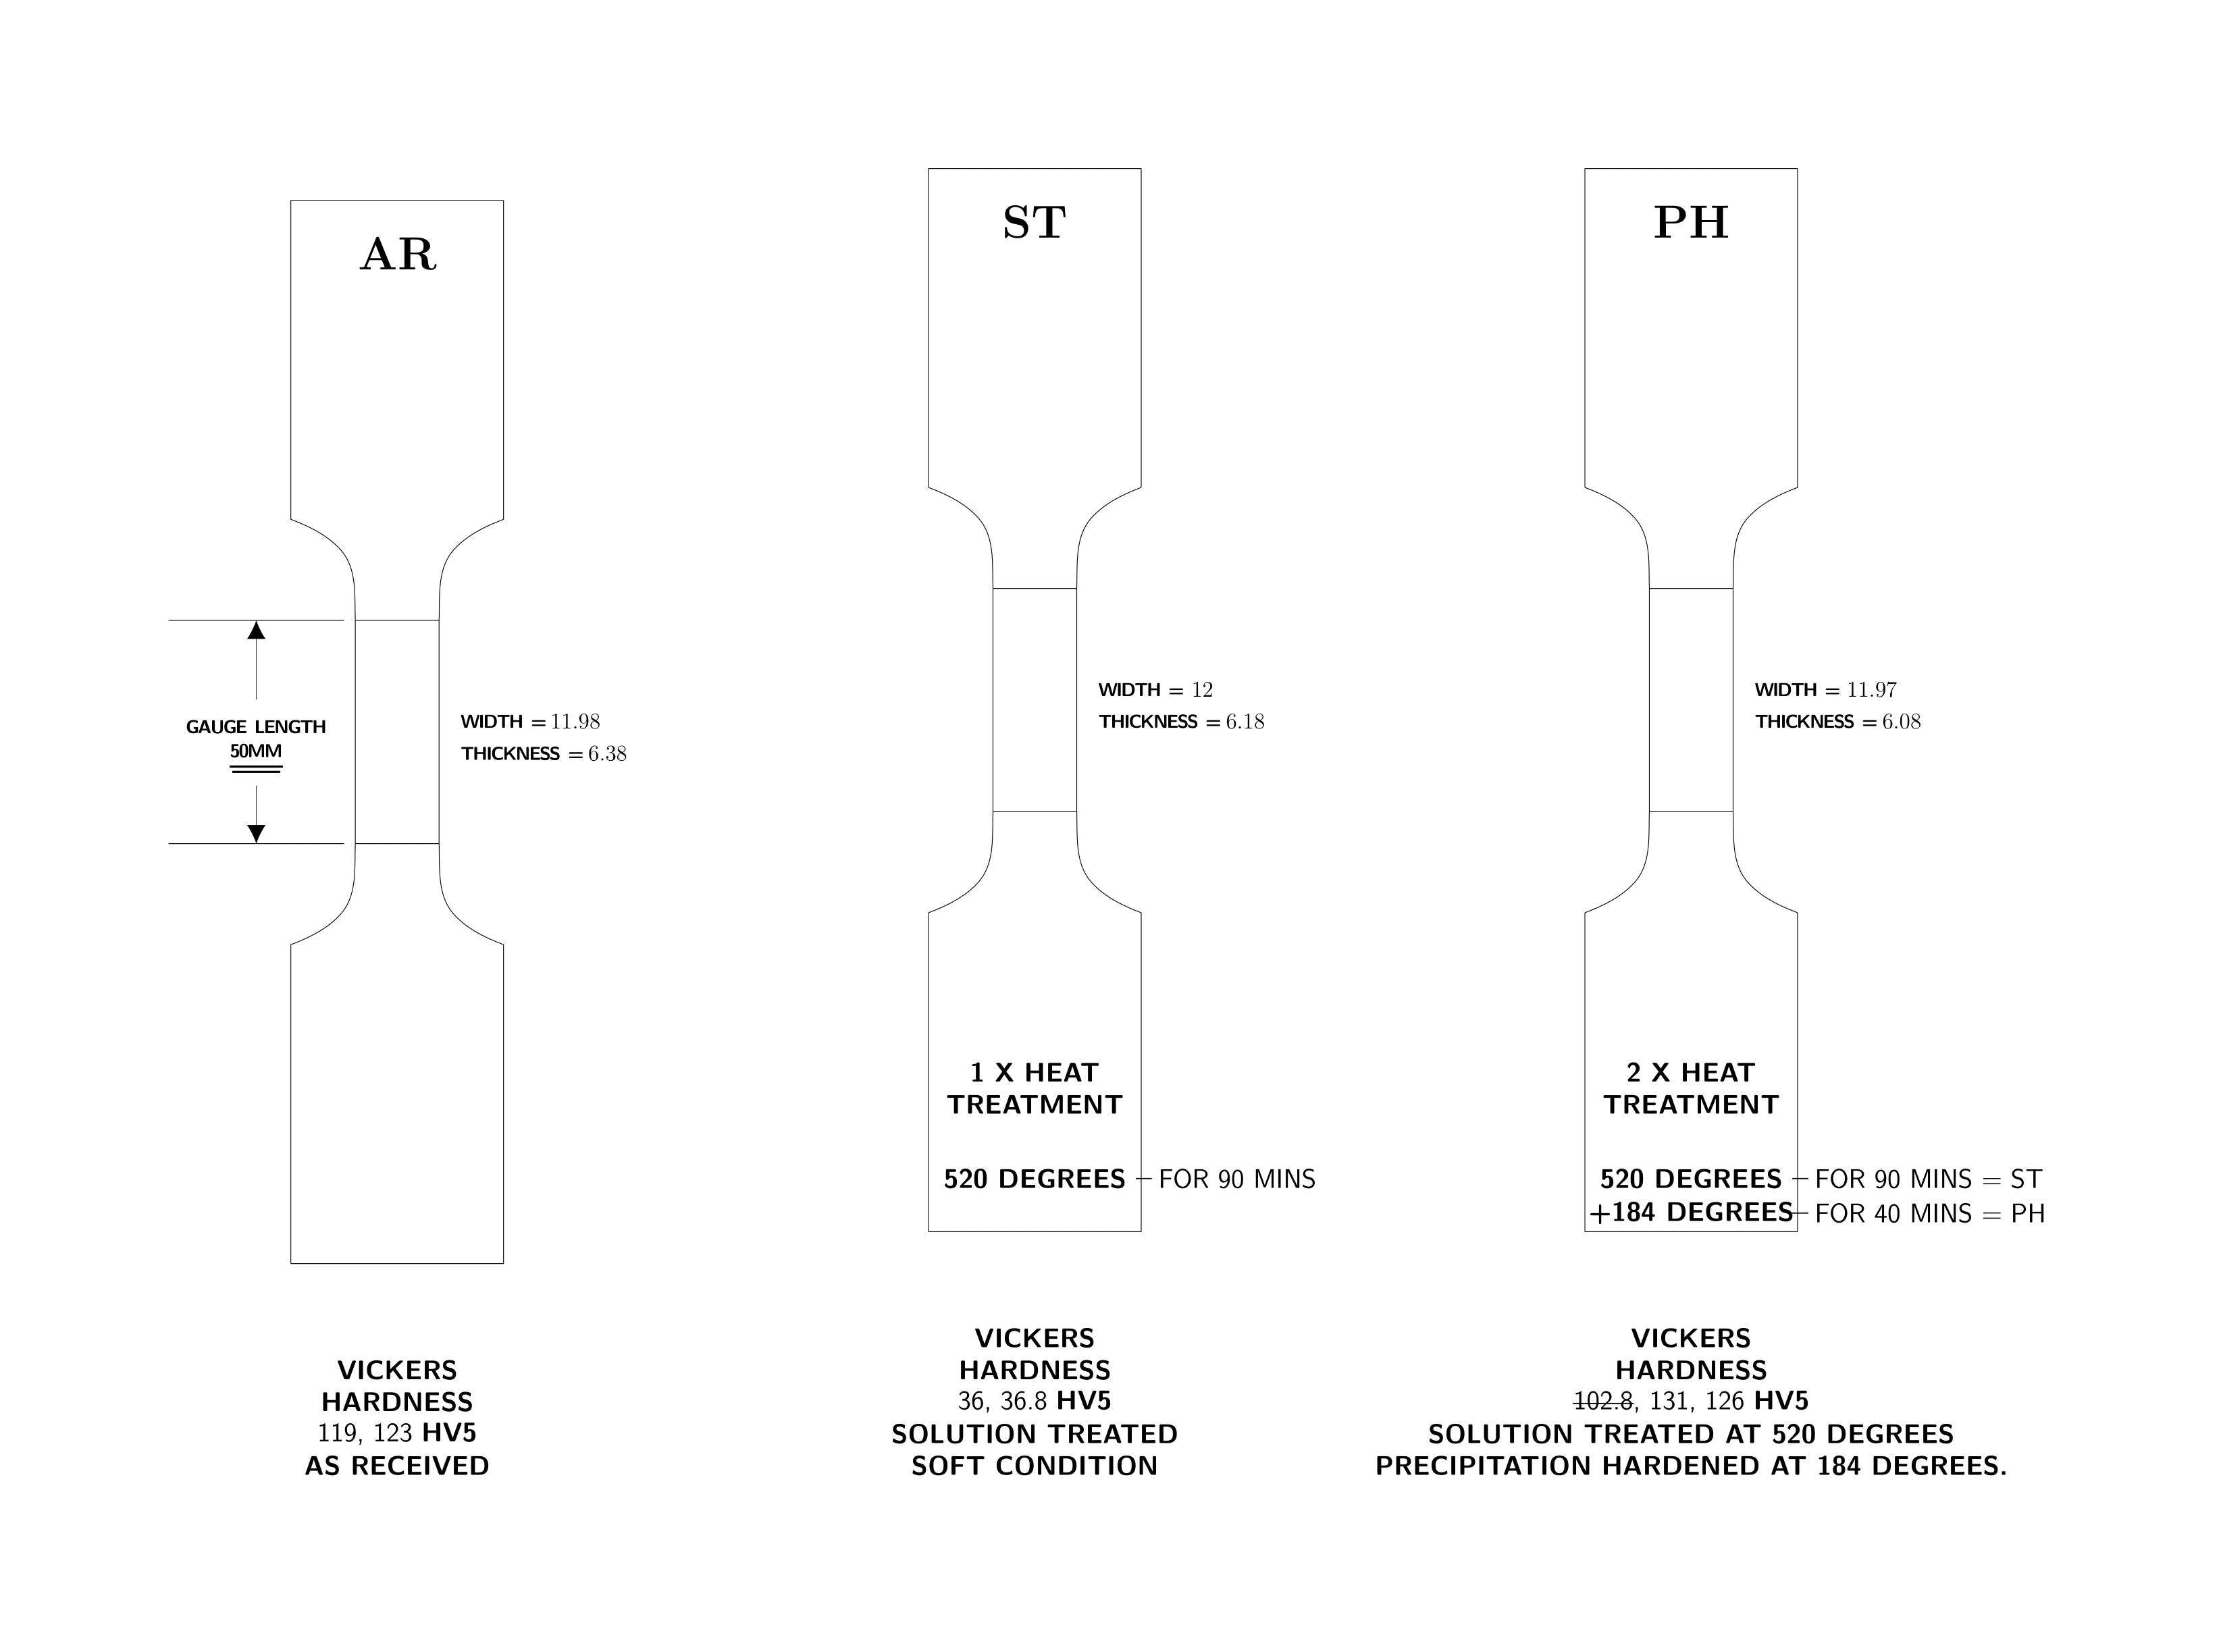
\includegraphics[width=\textwidth]{images/alloys.png}}
    \caption{alloys}
    \label{fig:alloys}
\end{figure}


\subsection{Equipment List}
The following equipment was used during the experiments:
\begin{itemize}
    \item \textbf{Digital Caliper}
    \item \textbf{Vickers Hardness Testing Machine}
    \item \textbf{Zwick Roell 2050 Tensile Testing Machine}
    \item \textbf{Personal Protective Equipment (PPE)}
    \item \textbf{Camera/Smartphone}
    \item \textbf{Miscellaneous Equipment}
\end{itemize}
\subsection{Risk Assessment}
The experimental procedures involved several potential hazards. The identified risks, their levels, and mitigation strategies are outlined below:
\begin{table}[h!]
    \centering
    \begin{tblr}{
            width=\linewidth,
            colspec={Q[4cm]Q[4cm]Q[2cm,c,m]Q[5cm]},
            row{1} = {font=\bfseries,c,m},
            rows,columns = {valign=m},
            hlines, vlines
        }
        Hazard & Risk & Level of Risk & Control Measures \\
        Sharp edges of dogbone samples & Cuts or injuries while handling samples & Medium & Handle with care; use gloves when measuring and mounting samples. \\
        Tensile testing machine & Pinching or crushing injuries from moving parts & High & Keep hands and body away from moving components during operation; follow machine's safety protocols. \\
        Vickers hardness testing machine & Injury from improper handling or sample misplacement & Medium & Ensure proper training before operation; position samples correctly and keep fingers clear. \\
        General laboratory environment & Slips, trips, and falls due to clutter or spills & Low & Maintain a tidy workspace; clean spills immediately; wear appropriate footwear. \\
    \end{tblr}
    \caption{Identified hazards, associated risks, levels, and control measures.}
    \label{tab:risk-assessment}
\end{table}

 


    \newpage\vspace*{-5pt}
    \section{Theory}

    \newpage\vspace*{-20pt}
    
    \section{Results}
        \renewcommand{\arraystretch}{1.4}
        \begin{table}[H]
            \centering
            \begin{tblr}{
                    width=\textwidth,
                    colspec={X[0.4,c]X[1,c]X[1.1,c]X[1.9,c]X[1.9,c]X[1.1,c]X[0.8,c]X[0.7,c]},
                    hlines,vlines,
                    cells={valign=m,halign=c}
                }
                \textbf{Nr} & \textbf{Specimen ID} & \textbf{Date} & \textbf{Stress - Maximum Load (N)} & \textbf{Strain Extension at Break (mm)} & \textbf{Thickness (mm)} & \textbf{Width (mm)} & \textbf{CSA \((\text{mm}^2)\)} \\
                1 & ST & 20/11/2024 & 8580 & 19.8 & 1 & 1 & 1.00 \\
                2 & PH & 20/11/2024 & 23800 & 9.8 & 1 & 1 & 1.00 \\
                3 & AR & 20/11/2024 & 24400 & 9.7 & 1 & 1 & 1.00 \\
                \end{tblr}
            \caption{Specimen Data}
            \label{tab:specimen_data}
        \end{table}

    \begin{figure}[H]
        \centering
        \includegraphics[scale=0.56]{figures/graph.png}
        \caption{Machine produced data}
        \label{fig:stress_strain}
    \end{figure}
    
    \newpage\vspace*{-5pt}
    \section{Discussion}

    \newpage\vspace*{-5pt}
    \section{Conclusions}

    \newpage\vspace*{-5pt}
    \section{Recommendations}

    \newpage\vspace*{-5pt}
    \section{References}
    \begin{enumerate}
        \item Singh, P., Singh, R.K. \& Das, A.K., (2023) \textit{‘Optimization of Heat Treatment Cycle for Cast-Al6082 Alloy to Enhance the Mechanical Properties‘}. Research Square. Available at: 	\url{https://assets-eu.researchsquare.com/files/rs-3363991/v1/9cd60f8c-a164-4e04-8552-1933478eaded.pdf?c=1711467707} [Accessed 7 December 2024]. 
    \end{enumerate}
    
    \newpage\vspace*{-5pt}
    
   
    
\section{Appendix}
\normalsize
\renewcommand{\thesubsection}{\Alph{subsection}}
\subsection{HV5 (Vickers Hardness - 5 kgf Load)}
The Vickers hardness test is a method for determining the hardness of materials using a diamond pyramid indenter. The hardness is calculated by dividing the applied force by the surface area of the indentation.\\[1em]
The general formula for calculating the Vickers Hardness Number (HV) is:
\begin{equation}
    HV = \frac{F}{A}
\end{equation}
Where:
\begin{itemize}[itemsep=-1mm]
    \item \( F \) : applied force in newtons (N),
    \item \( A \) : surface area of the indentation in square millimeters (mm\(^2\)).
\end{itemize}
For the HV5 test, the applied load is fixed at 49.03 N. Therefore, the formula for HV5 becomes:
\begin{equation}
    HV_5 = \frac{49.03}{A}
\end{equation}
Where:
\begin{itemize}[itemsep=-1mm]
    \item \( 49.03 \) N is the fixed applied force for HV5,
    \item \( A \) is the surface area of the indentation in mm\(^2\).
\end{itemize}
This formula quantifies the material's hardness by calculating the force applied per unit area of the indentation. The surface area \( A \) is determined based on the geometry of the diamond pyramid indenter used in the test.
\subsection{BHN (Brinell Hardness Number)}
The Brinell Hardness Number (BHN) measures a material's resistance to deformation, determined by the indentation left by a hard steel or carbide ball pressed into the material under a specified load. This test is commonly used for materials with a coarse or heterogeneous grain structure.\\[1em]
The formula for calculating the Brinell Hardness Number is:

\begin{equation}
    BHN = \frac{2P}{\pi D (D - \sqrt{D^2 - d^2})}
\end{equation}
Where:
\begin{itemize}[itemsep=-1mm]
    \item \( P \) : applied load in kilogram-force (kgf),
    \item \( D \) : diameter of the indenter (typically 10 mm),
    \item \( d \) : diameter of the indentation (mm).
\end{itemize}
The BHN provides insight into a material's ability to resist wear and deformation, which is important for assessing the durability and suitability of metals in various engineering applications. BHN values are particularly useful for testing larger, rougher materials and are commonly applied to metals like steel and cast iron. The results help predict wear resistance and strength under load.

\end{document}
